\begin{appendices} % Do not change this line (if you have appendices). 
                   % Otherwise, completely delete the contents of this file



	\section{Обоснование метода}

        Из определения модели имеем три уравнения:
        \begin{equation} \label{rp1}
                A_{t_k} = V_{t_k} + \frac{s}{2} + \sum _{i=0} ^{k-1} x_{t_i} \kappa e^{- \rho (t_k - t_i)}
        \end{equation}
        \begin{equation}\label{rp2}
                V_{t_{k+1}} = V_{t_k} + \lambda x_{t_k} \rightarrow V_{t_{k+1}} - V_{t_k} = \lambda x_{t_{k}}
        \end{equation}
        \begin{equation} \label{rp3}
                D_{t_k} = A_{t_k} - V_{t_k} - \frac{s}{2}
        \end{equation}
        Следующее замечание является основополагающим в нашей методологии подбора параметра $\rho$.
        Здесь и далее $\Delta t_{k+1} := t_{k+1} - t_k, \Delta A_{k+1} := A_{k+1} - A_k$.
        \begin{lemma} \label{mainregrOW}
                В модели Обижаевой-Ванга:
                \begin{equation*}
                        \Delta A_k = D_{t_k} (e^{- \rho \Delta t_k} - 1) + x_{t_k} \kappa e^{- \rho \Delta t_k} + \lambda x_{t_k} .
                \end{equation*}
        \end{lemma}
        \begin{proof}
                Сперва покажем, что 
                \begin{equation*} \label{DeltaDk}
                    \Delta D_{k} = D_{t_k} (e^{- \rho \Delta t_k} - 1) + x_{t_k} \kappa e^{- \rho \Delta t_k}.
                \end{equation*}
                Пользуясь \eqref{rp1} и \eqref{rp3}, получаем
                \begin{align*}
                        D_{t_k} &= \sum _{i=0} ^{k-1} x_{t_i} \kappa e^{- \rho (t_k - t_i)} \\
                        \Delta D_{k} &= \sum _{i=0} ^k x_{t_i} \kappa e^{- \rho (t_{k+1} - t_i)} 
                        - \sum _{i=0} ^{k - 1} x_{t_i} \kappa e^{- \rho (t_k - t_i)}
                        = \sum _{i=0} ^{k - 1} x_{t_i} \kappa (e^{- \rho (t_{k+1} - t_i)} - e^{- \rho (t_k - t_i)})
                        + x_{t_k} \kappa e^{- \rho (t_{k+1} - t_k)} = \\
                        &= \sum _{i=0} ^{k - 1} x_{t_i} \kappa e^{- \rho (t_k - t_i)} (e^{- \rho (t_{k+1} - t_k)} - 1)
                        + x_{t_k} \kappa e^{- \rho (t_{k+1} - t_k)} = D_{t_k} (e^{- \rho \Delta t_k} - 1) + x_{t_k} \kappa e^{- \rho \Delta t_k}.
                \end{align*}
                Теперь покажем, что 
                \begin{equation*}
                        \Delta A_k = D_{t_k} (e^{- \rho \Delta t_k} - 1) + x_{t_k} \kappa e^{- \rho \Delta t_k} + \lambda x_{t_k} .
                \end{equation*}
                Из \eqref{rp2} и \eqref{rp3} имеем
                \begin{equation*}
                        \Delta D_k = D_{t_{k+1}} - D_{t_k} = A_{t_{k+1}} + V_{t_{k+1}} - A_{t_k} - V_{t_k} = \Delta A_k - \Delta V_k.
                \end{equation*}
                Отсюда имеем, что 
                \begin{equation*}
                        \Delta A_k = \Delta D_k + \Delta V_k .
                \end{equation*}
                Подставив сюда \eqref{DeltaDk}, получаем утверждение леммы. 
        \end{proof}

        Мы считаем, что при всей своей простоте оно очень ценно, поскольку даёт путь к выводу регрессионного уравнения.

        \begin{theorem} \label{GenIntT}
                Интерполируя экспоненту в выражении 
                \begin{equation*} \label{DeltaDk}
                        \Delta D_{k} = D_{t_k} (e^{- \rho \Delta t_k} - 1) + x_{t_k} \kappa e^{- \rho \Delta t_k}.
                \end{equation*}
                функцией вида $e^{- \rho \Delta t_k} = 1 - B \rho \Delta t_k + E(\rho \Delta t_k) $, где $E(\rho \Delta t_k)$ ---
                ошибка интерполяции,
                можно получить регрессионное уравнение вида:
                \begin{align*}
                        & \frac{\Delta A_{k+1}}{\Delta t_{k+1}} - \frac{\Delta A_{k}}{\Delta t_{k}} = 
                        -B \Delta A_k + B (\lambda + \kappa) x_{t_k} - B \kappa x_{t_{k+1}} 
                        + (\lambda + \kappa) \left(\frac{x_{t_{k+1}}}{\Delta t_{k+1}} - \frac{x_{t_k}}{\Delta t_{k}}\right) + E (\rho \Delta t_{k+1}) - E (\rho \Delta t_k).
                \end{align*}  
        \end{theorem}
        \begin{proof}
                Пусть $f(\rho \Delta t_k)$ --- некоторая функция, приближающая экспоненту с ошибкой $(\rho \Delta t_k)$.
                Тогда, подставив эту функцию в уравнение \eqref{mainregrOW}, получаем
                \begin{equation*}
                        \frac{\Delta A_k}{\Delta t_k} = D_{t_k} (\frac{f(\rho \Delta t_k) - 1}{\Delta t_k}) 
                        + x_{t_k} \kappa {\frac{f(\rho \Delta t_k)}{\Delta t_k}} + \lambda \frac{x_{t_k}}{\Delta t_k} . 
                \end{equation*}
                Потребуем, чтобы при рассмотрении разности $\frac{\Delta A_{k+1}}{\Delta t_{k+1}} - \frac{\Delta A_k}{\Delta t_k}$ 
                выполнялось условие 
                $\frac{f(\rho \Delta t_{k+1}) - 1}{\Delta t_{k+1}} = \frac{f(\rho \Delta t_k) - 1}{\Delta t_k}$. В этом случае, 
                рассматривая разность делённых на время асков, можно
                исключить из уравнения ненаблюдаемый временной ряд $D_{t_k}$:
                \begin{align*}
                        & R := (x_{t_{k+1}} \kappa + D_{t_{k+1}}) \frac{E(\rho \Delta t_{k+1})}{\Delta t_{k+1}} -
                         (x_{t_k} \kappa + D_{t_k}) \frac{E(\rho \Delta t_k)}{\Delta t_k} \\
                        \frac{\Delta A_{k+1}}{\Delta t_{k+1}} - \frac{\Delta A_{k}}{\Delta t_{k}} &=
                        - B D_{t_{k+1}} + x_{t_{k+1}} \kappa \left(\frac{1}{\Delta t_{k+1}} - \rho \right) + \lambda \frac{x_{t_{k+1}}}{\Delta t_{k+1}}
                        + B D_{t_{k}}   - x_{t_{k}}   \kappa \left(\frac{1}{\Delta t_{k}} - \rho \right)   - \lambda \frac{x_{t_k}}    {\Delta t_{k}} 
                        + R = \\
                        &= -B (\Delta A_k - \Delta V_k) + (\lambda + \kappa) \left(\frac{x_{t_{k+1}}}{\Delta t_{k+1}} - \frac{x_{t_k}}{\Delta t_{k}}\right) 
                        - B \kappa (x_{t_{k+1}} - x_{t_{k}}) + R = \\
                        &= -B \Delta A_k + B (\lambda + \kappa) x_{t_k} - B \kappa x_{t_{k+1}} 
                        + (\lambda + \kappa) \left(\frac{x_{t_{k+1}}}{\Delta t_{k+1}} - \frac{x_{t_k}}{\Delta t_{k}}\right) + R.
                \end{align*} 

        \end{proof}
        \par
        Помимо всего прочего, в доказательстве показано, что такой подход к выводу регрессионного уравнения 
        не работает ни для какого более широкого класса непрерывных или монотонных функций, чем двучлены вида 
        $1 - B \rho \Delta t_k$,
        поскольку единственной непрерывной или монотонной функцией одной переменной, обладающей свойством
        однородности первой степени, необходимым для осуществления рассуждения выше, является функция 
        $g(\rho \Delta t_k) = f(\rho \Delta t_k) - 1 = - B \rho \Delta t_k $. 
        \par
        Впрочем, это не исключает возможности того, что существует иной путь вывода регрессионого уравнения,
        позволяющий рассмотреть более точную интерполяцию. Это интересный вопрос для отдельного исследования.  
        
        \begin{theorem}\label{lilreg}
                В регрессии                                                                                                                                                                                                                                                                                                                                                                                       
                \begin{equation*}
                        \frac{\Delta A_{k+1}}{\Delta t_{k+1}} - \frac{\Delta A_{k}}{\Delta t_{k}}
                        = -B \Delta A_k + B (\lambda + \kappa) x_{t_k} - B \kappa x_{t_{k+1}} + 
                        (\lambda + \kappa) \left(\frac{x_{t_{k+1}}}{\Delta t_{k+1}} - \frac{x_{t_k}}{\Delta t_{k}}\right),
                \end{equation*}
                где $x_{k}$ и $A_{k}$ --- глубина ордера и аск в момент времени $t_k$, соответственно, \\
                $\rho = B + O(\rho^2 \Delta t)$ .
        \end{theorem}
        \begin{proof}
        Разложим экспоненту в ряд Тейлора: 
        \begin{equation*}
                e^{- \rho \Delta t_k} = 1 - \rho \Delta t_k + (\rho \Delta t_k) ^2 \sum_{i=0}^{\infty} \frac{(\rho \Delta t_k)^i}{(i+2)!},
        \end{equation*}
        тогда из \ref{GenIntT}, получим:
        \begin{align*}
                & R := (x_{t_{k+1}} \kappa + D_{t_{k+1}}) \rho^2 \Delta t_{k+1}  \sum_{i=0}^{\infty} \frac{(\rho \Delta t_{k+1})^i}{(i+2)!} 
                - (x_{t_k} \kappa + D_{t_k}) \rho^2 \Delta t_k \sum_{i=0}^{\infty} \frac{(\rho \Delta t_k)^i}{(i+2)!} \\
                & \frac{\Delta A_{k+1}}{\Delta t_{k+1}} - \frac{\Delta A_{k}}{\Delta t_{k}} = -\rho \Delta A_k + \rho (\lambda + \kappa) x_{t_k} - \rho \kappa x_{t_{k+1}} 
                + (\lambda + \kappa) \left(\frac{x_{t_{k+1}}}{\Delta t_{k+1}} - \frac{x_{t_k}}{\Delta t_{k}}\right) + R.
        \end{align*} 
        \end{proof}
        % Полагая, что $e^{- \rho \Delta t_k} = 1 - \rho \Delta t_k + \frac{1}{2} (\rho \Delta t_k)^2 + o((\rho \Delta t_k) ^3)$, имеем:
        % \begin{align*}
        %         \Delta D_{t_k} &=  D_{t_k} (e^{- \rho \Delta t_k} - 1) + x_{t_k} \kappa e^{- \rho \Delta t_k} 
        %         =  - \rho D_{t_k} \Delta t_k + x_{t_k} \kappa (1 - \rho \Delta t_k) + (x_{t_k} \kappa + D_{t_k}) o((\rho \Delta t_k) ^3) 
        % \end{align*}

        \section{Что делать, если $\rho$ получается большим?} \label{AppendixBigRho}

        Теорема \ref{lilreg} даёт указание к действию, когда $\rho^2 \Delta t$ мал. Но что делать, если это условие систематически 
        нарушается, например, актив настолько ликвиден, что $\rho$ существенно превосходит единицу? \par
        % Если предположить, что данные действительно подчинены экспоненциальному закону, то, в такой постановке, метод наименьших 
        % квадратов фактически будет решать задачу:
        % \begin{equation*}
        %         \sum _{i} \Delta t_i \left(e^{- \rho \Delta t_i} - 1 + B \Delta t_i \right) \rightarrow \min.
        % \end{equation*} 
        % Её решение легко найти аналитически:
        % \begin{equation*}
        %         B = \frac{\sum _{i} \Delta t_i}{\sum _{i} \Delta t_i^2} - \frac{\sum _{i} \Delta t_i e^{-\rho \Delta t_i}}{\sum _{i} \Delta t_i^2} 
        %         = \frac{\sum _{i} \Delta t_i ( 1 - e^{-\rho \Delta t_i})}{\sum _{i} \Delta t_i^2}.
        % \end{equation*} 
        % При $\rho \Delta t_i \rightarrow 0$ имеем $1 - e^{-\rho \Delta t_i} \rightarrow \rho \Delta t_i$, 
        % а значит, $B \rightarrow \rho$, то есть такой подход подтверждает и расширяет полученный ранее вывод. 
        % Однако, эта формула очень неудобна для численного вычисления $\rho(B)$ в иных случаях. Поэтому будем считать,
        % что при вычисленнии коэффициентов решается задача
        
        \begin{theorem}
                Если считать, что при большом $\rho \Delta t$ регрессия решает задачу
                \begin{equation*}
                        \min _{B \in \mathbb{R}} \max _{x \in [0, t_0]} |e^{- \rho x} - 1 + B x|,
                \end{equation*} 
                где $t_0$ некоторое "среднее" время между двумя соседними ордерами, то $B$ и $\rho$ связаны уравнением:
                \begin{equation*}
                        2 - \frac{B}{\rho}\left(1 - \ln \frac{B}{\rho}\right) = e^{- \rho t_0} + B t_0.
                \end{equation*} 
        \end{theorem}
        \begin{proof}
        Очевидно, разность под модулем обращается в ноль в двух точках ($0$ и $x_0$), если только прямая не является касательной к экспоненте.
        При этом, функция выпукла в промежутке $[0, x_0]$, а значит имеет там единственную точку экстремума. Из свойств функции ясно, что $B$ 
        является решением задачи в том и только в том случае, когда:
        \begin{equation*}
                - extr \{e^{-\rho x} - 1 + B x \}_{x \in [0, x_0]} = e^{-\rho t_0} - 1 + B t_0.
        \end{equation*} 
        Легко найти точку экстремума $x_*$:
        \begin{equation*}
                \frac{d}{dx} \Big| _{x=x_*} (e^{-\rho x} - 1 + B x) = 0 \rightarrow -\rho e^{-\rho x_*} + B = 0 \rightarrow x_* = -\frac{1}{\rho} \ln \frac{B}{\rho}.
        \end{equation*} 
        Отсюда получаем уравнение, связывающее $\rho$ и $B$:
        \begin{equation*}
                2 - \frac{B}{\rho}\left(1 - \ln \frac{B}{\rho}\right) = e^{- \rho t_0} + B t_0.
        \end{equation*} 
        \end{proof}
        \textit{Замечание.} Сделаем замены $\rho x = B, t_0 B = y$, тогда уравнение примет вид:
        \begin{equation*}
                2 - x \left(1 - \ln x\right) = e^{- \frac{y}{x}} + y.
        \end{equation*} 
        После замен $\rho x = B, t_0 \rho = y$ уравнение примет вид:
        \begin{equation*}
                2 - x \left(1 - \ln x\right) = e^{- y} + x y.
        \end{equation*} 
        Такие представления уравнений могут быть использованы для исследования связи $\rho$ и $B$. Например, в случае когда $B$ велико и,
        как следствие, не выполнено условие теоремы \ref{lilreg}, в некоторых случаях благодаря предположениям на $y$ мы можем получить оценку
        $x$. Если $B / x$ велико, то можно утверждать, что $\rho$ велико по модулю. В этом случае, стратегия оптимального исполнения вырождается в
        TWAP.


        % Наконец, мы получили искомое уравнение
        % \begin{equation*}
        %         \frac{\Delta A_{k+1}}{\Delta t_{k+1}} - \frac{\Delta A_{k}}{\Delta t_{k}} = 
        %         -\rho \Delta A_k + \rho (\lambda + \kappa) x_{t_k} - \rho \kappa x_{t_{k+1}} + (\lambda + \kappa) \left(\frac{x_{t_{k+1}}}{\Delta t_{k+1}} - \frac{x_{t_k}}{\Delta t_{k}}\right).
        % \end{equation*}
	

        \section{Время между сделками} \label{timedistr}
        Здесь, на рисунках \ref{appstart}--\ref{append}, представлены распределения времён между сделками для всех исследуемых активов.

        \begin{figure}
                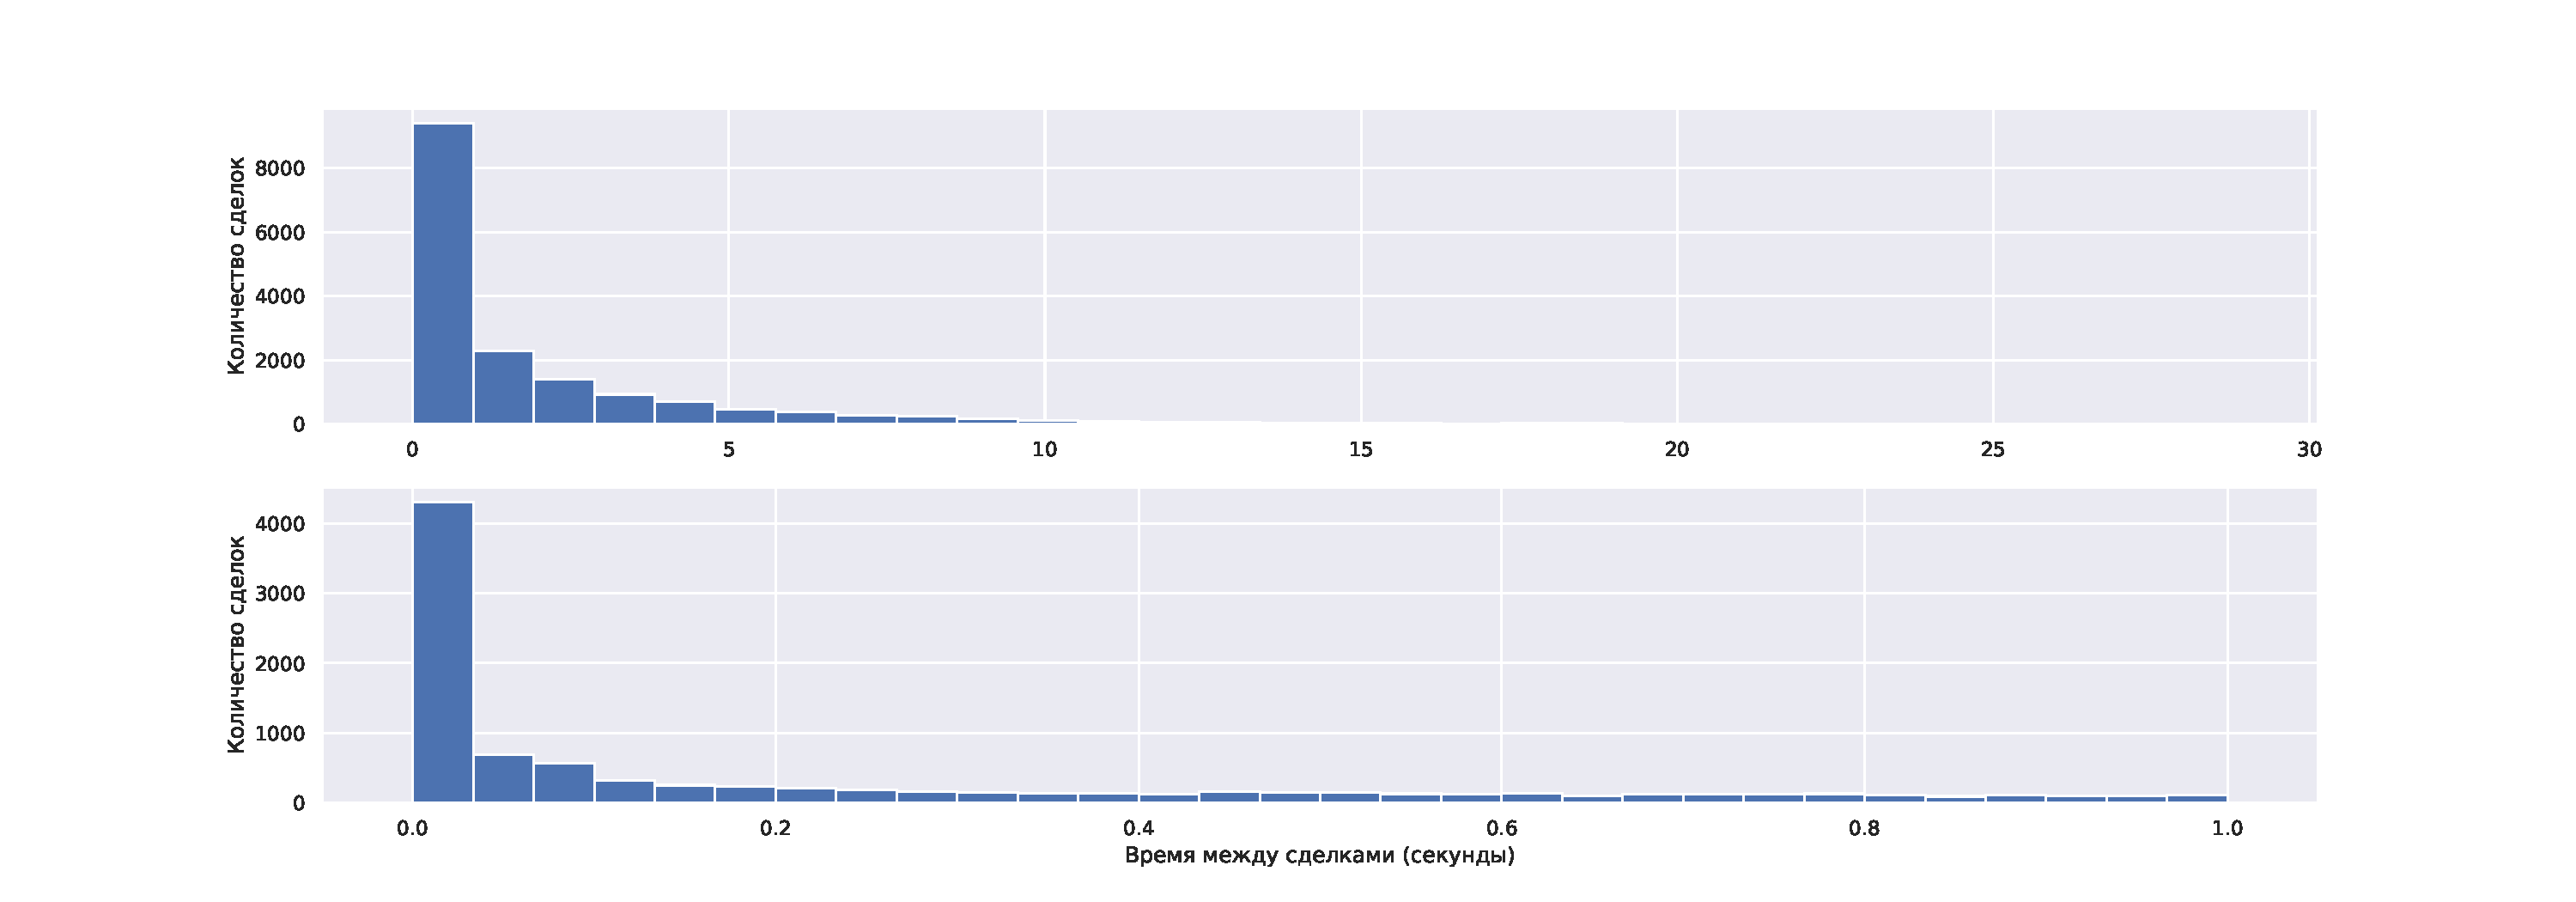
\includegraphics[scale=0.35]{fig/timedistr/SE/YNDX.pdf}
                \caption{Распределение времени между сделками для YNDX}
                \label{appstart}
        \end{figure}
        \begin{figure}
                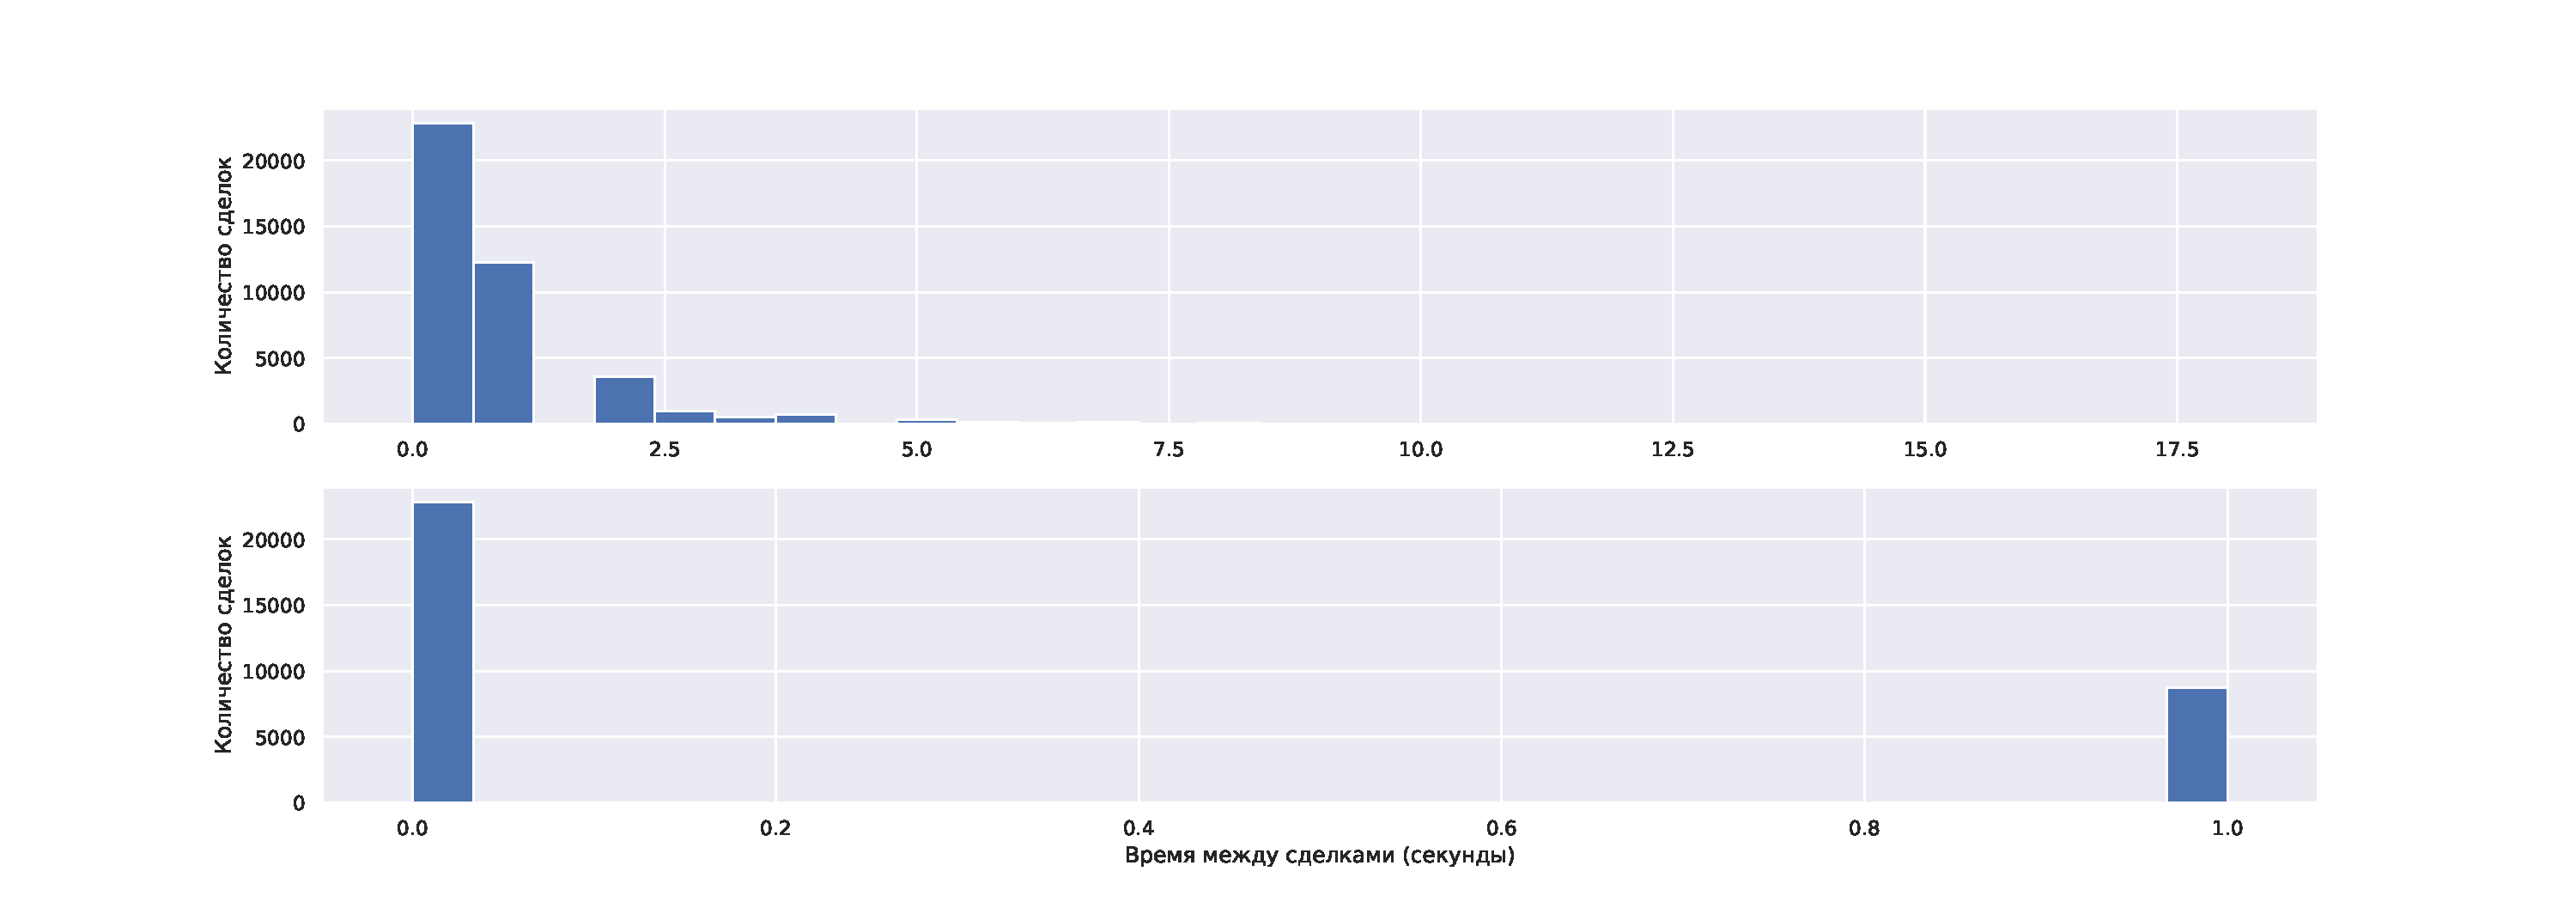
\includegraphics[scale=0.35]{fig/timedistr/SE/SBER.pdf}
                \caption{Распределение времени между сделками для SBER}
                \label{app}
        \end{figure}
        \begin{figure}
            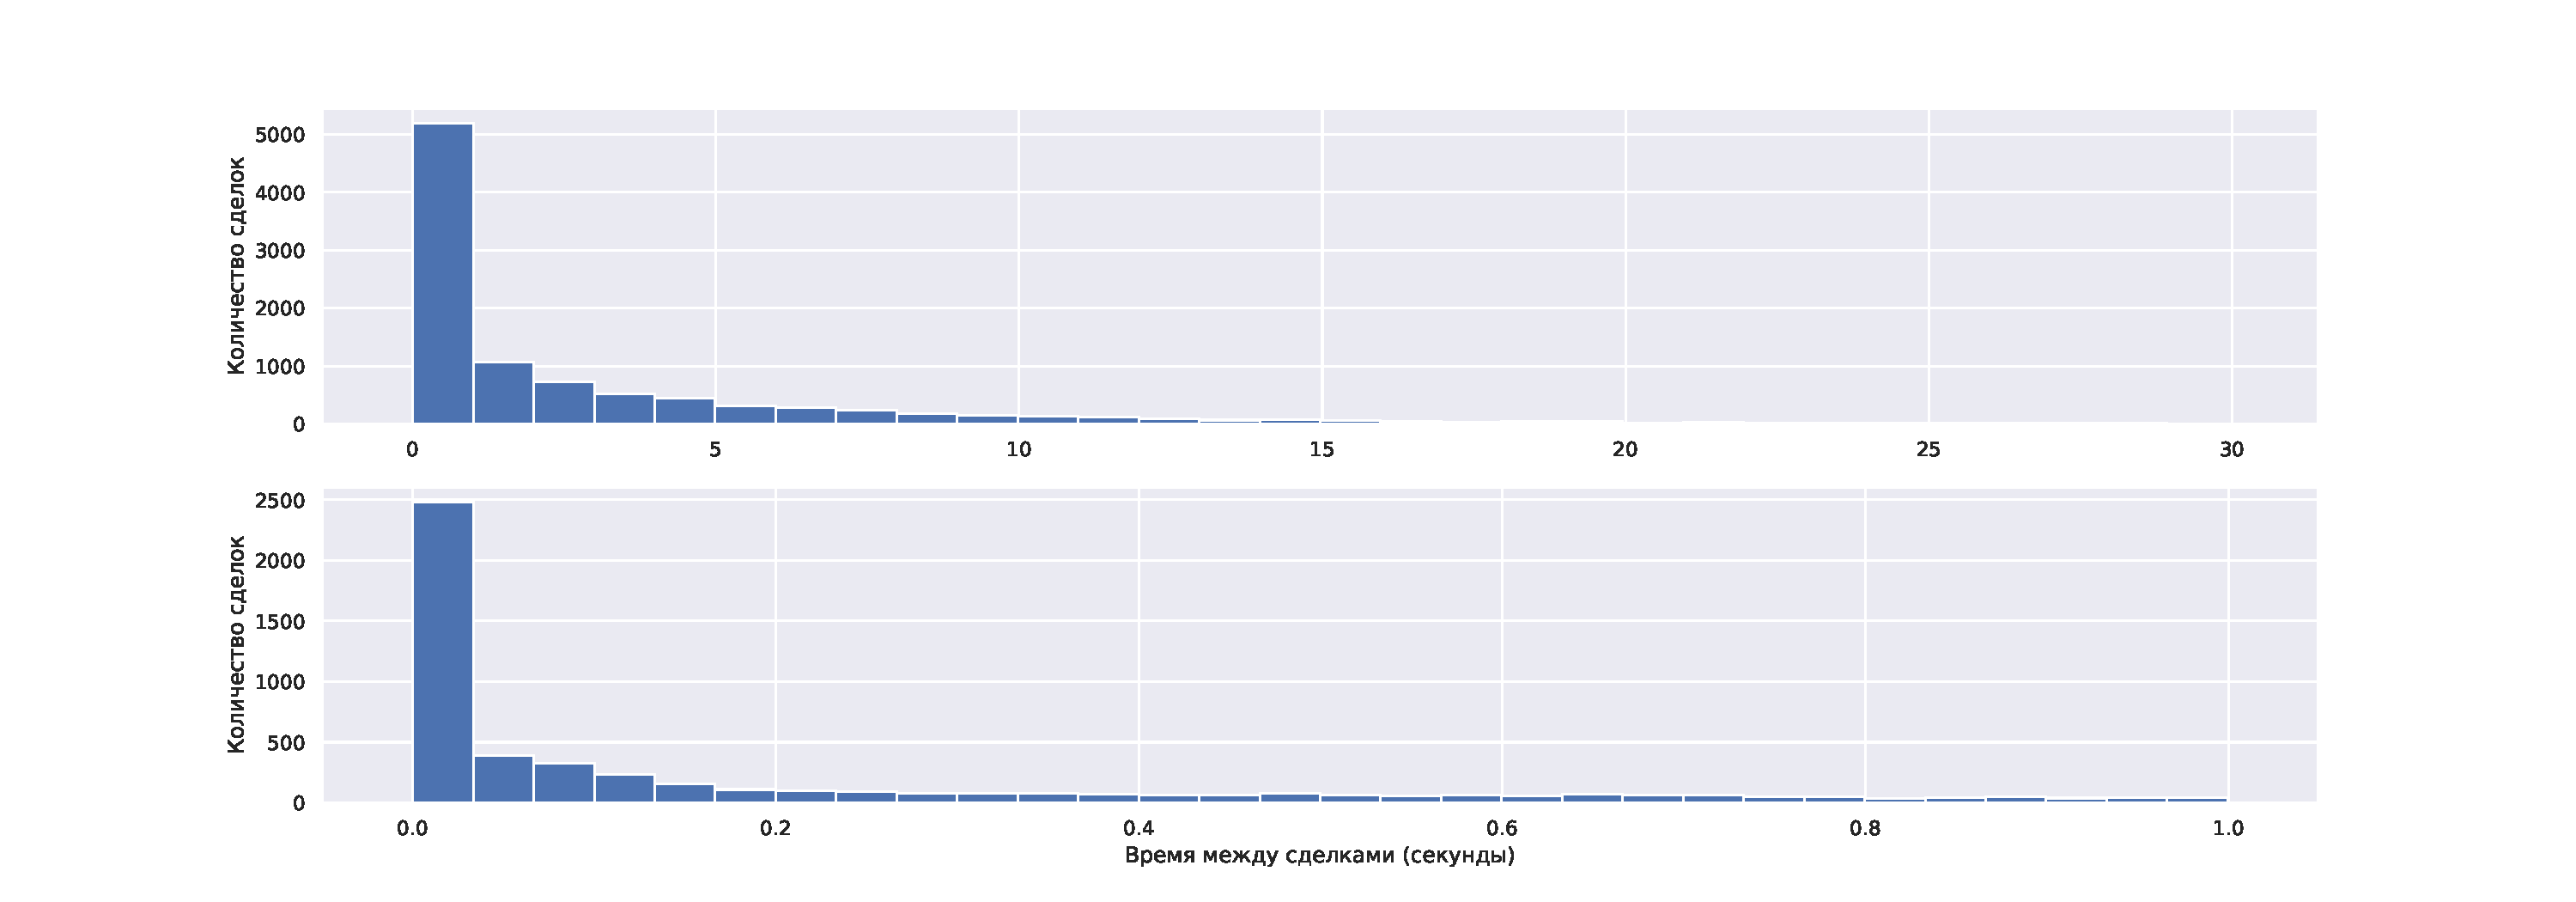
\includegraphics[scale=0.35]{fig/timedistr/SE/ROSN.pdf}
            \caption{Распределение времени между сделками для ROSN}
            \label{app}
        \end{figure}
        \begin{figure}
                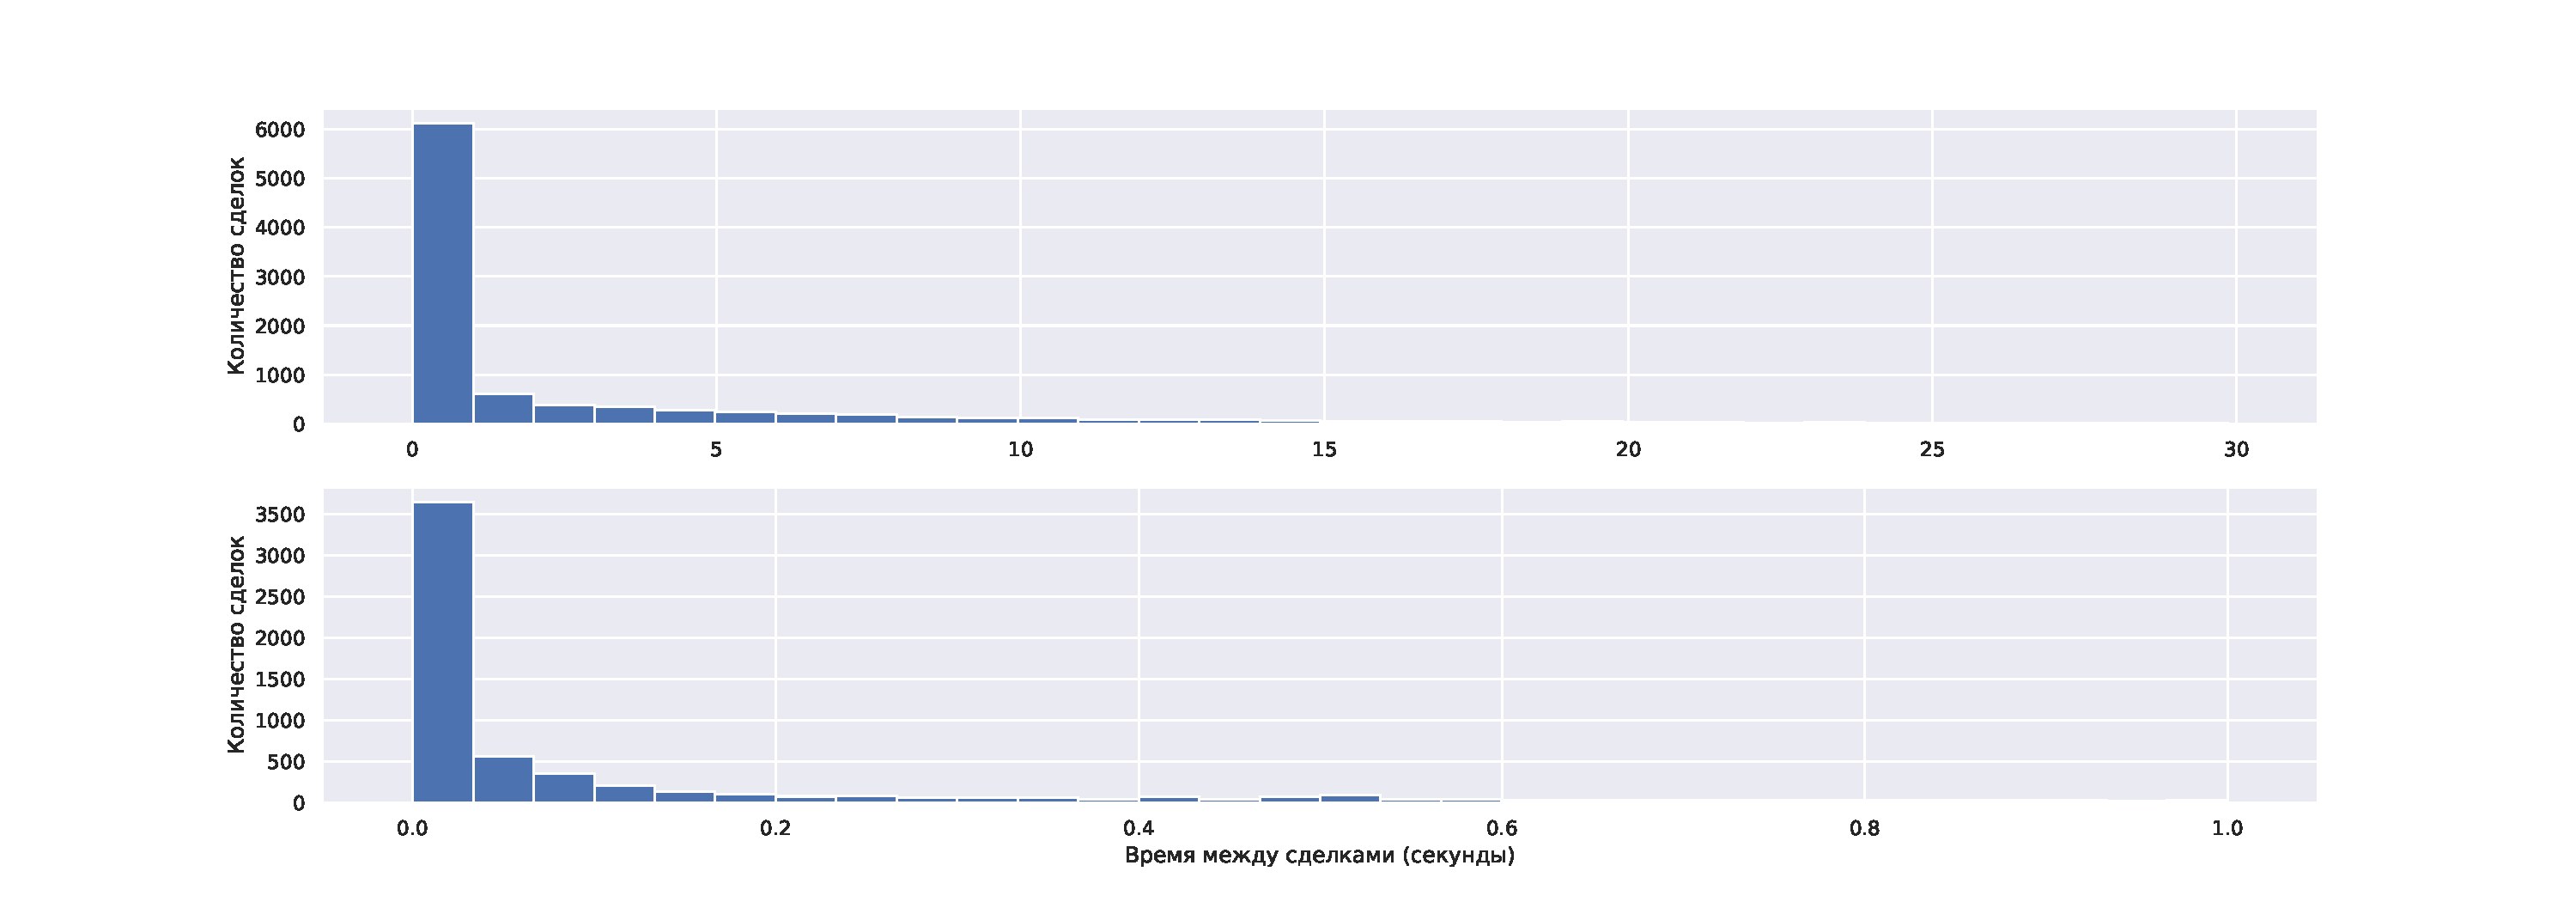
\includegraphics[scale=0.35]{fig/timedistr/SE/PLZL.pdf}
                \caption{Распределение времени между сделками для PLZL}
                \label{app}
        \end{figure}
        \begin{figure}
                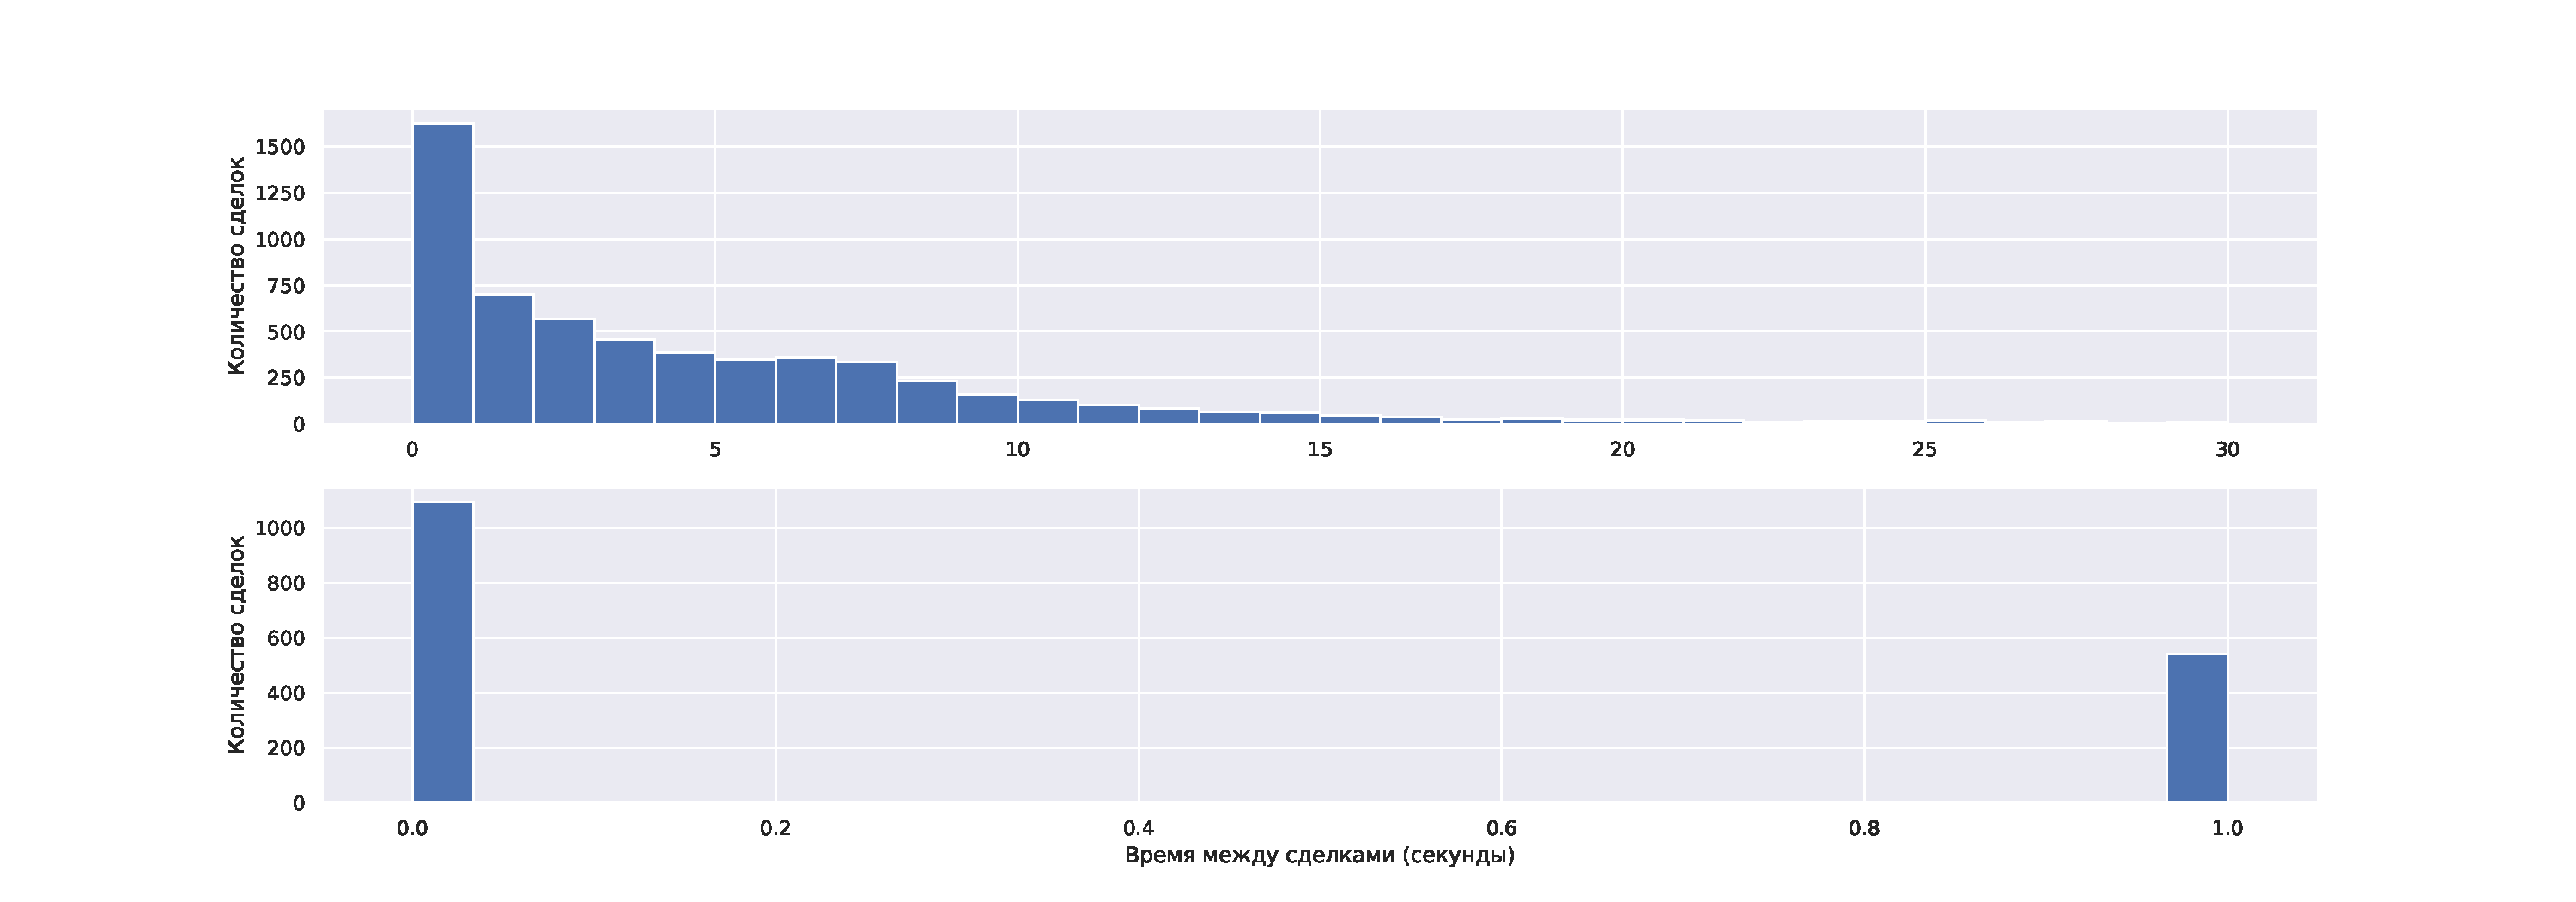
\includegraphics[scale=0.35]{fig/timedistr/SE/MTLR.pdf}
                \caption{Распределение времени между сделками для MTLR}
                \label{app}
        \end{figure}
        \begin{figure}
            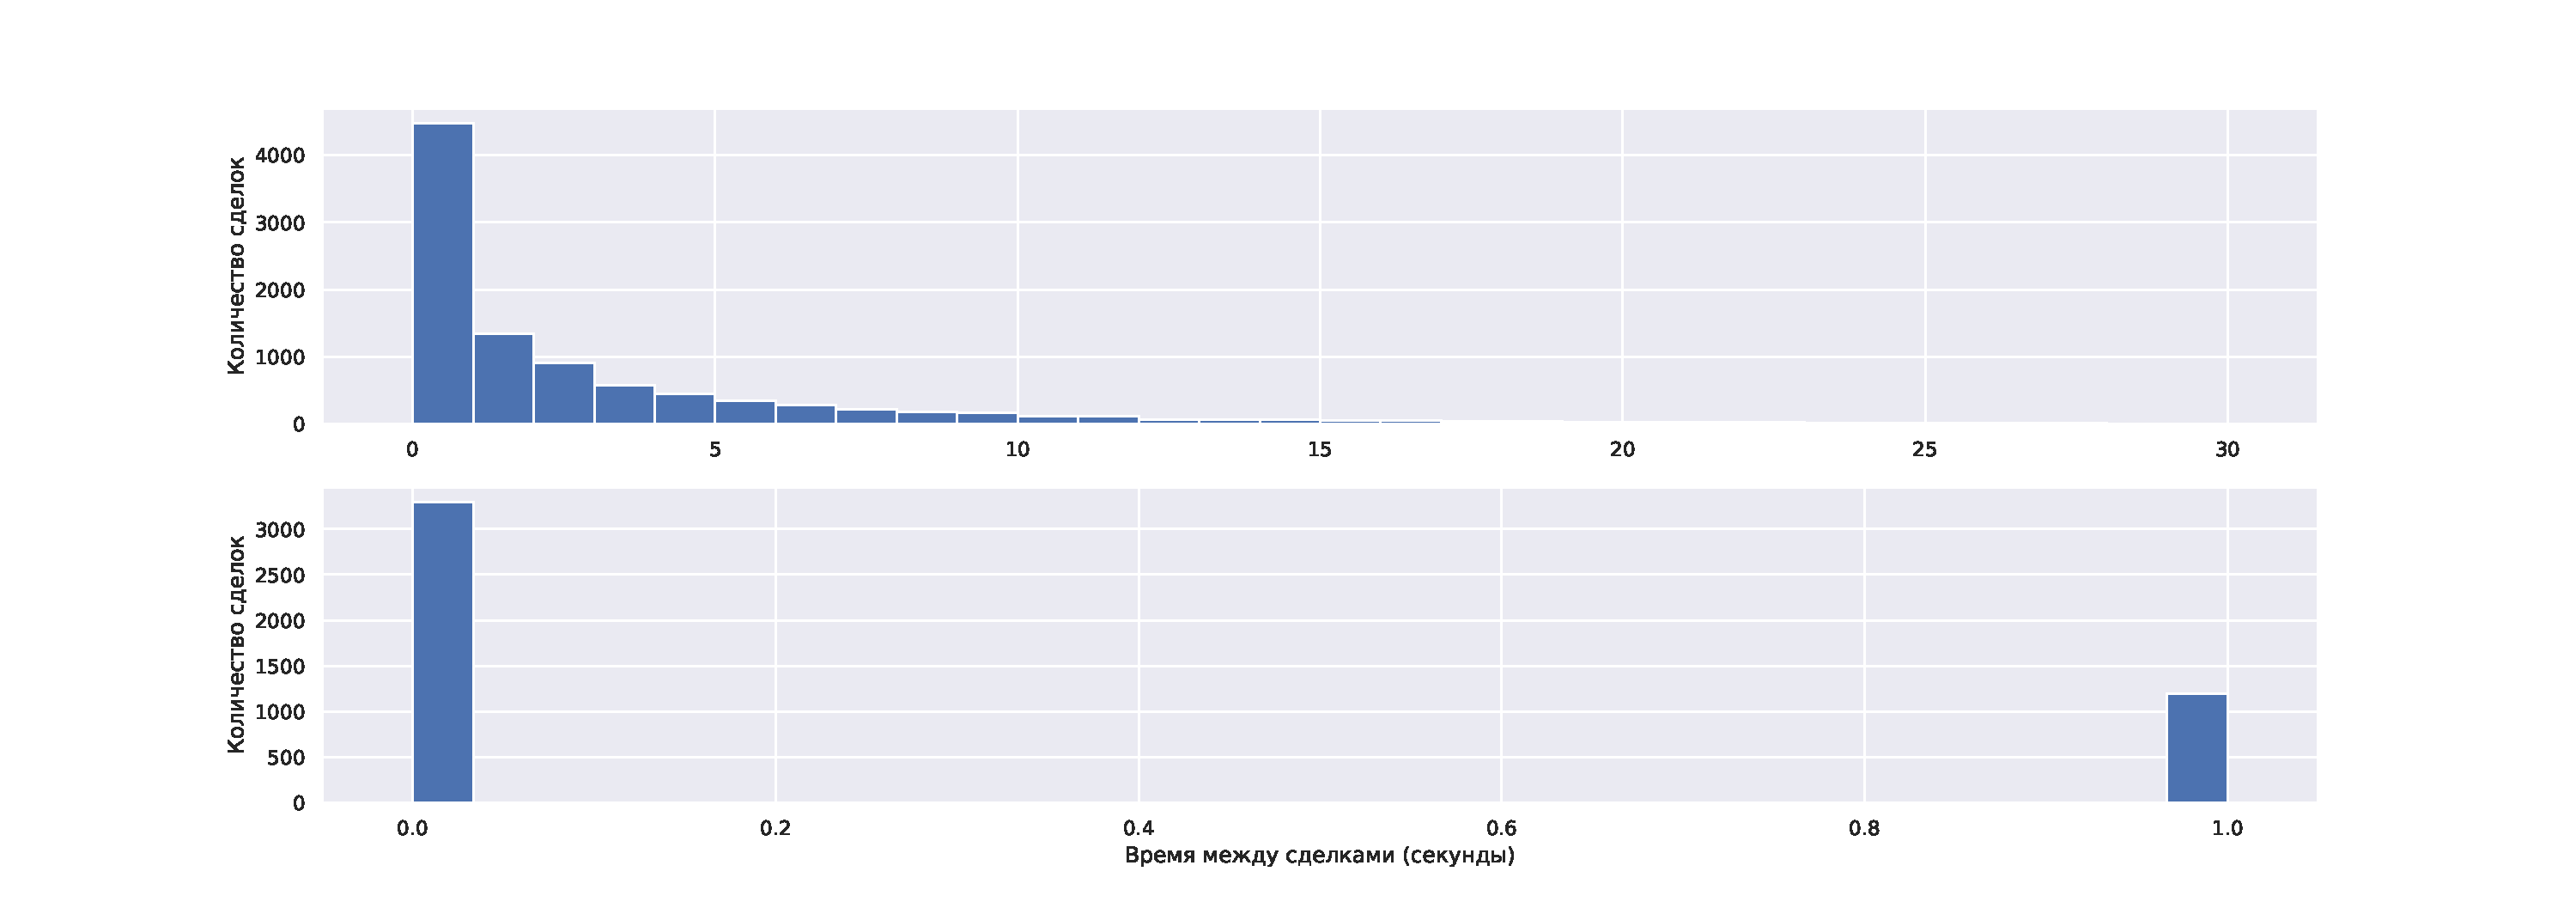
\includegraphics[scale=0.35]{fig/timedistr/SE/LKOH.pdf}
            \caption{Распределение времени между сделками для LKOH}
            \label{app}
        \end{figure}
        \begin{figure}
                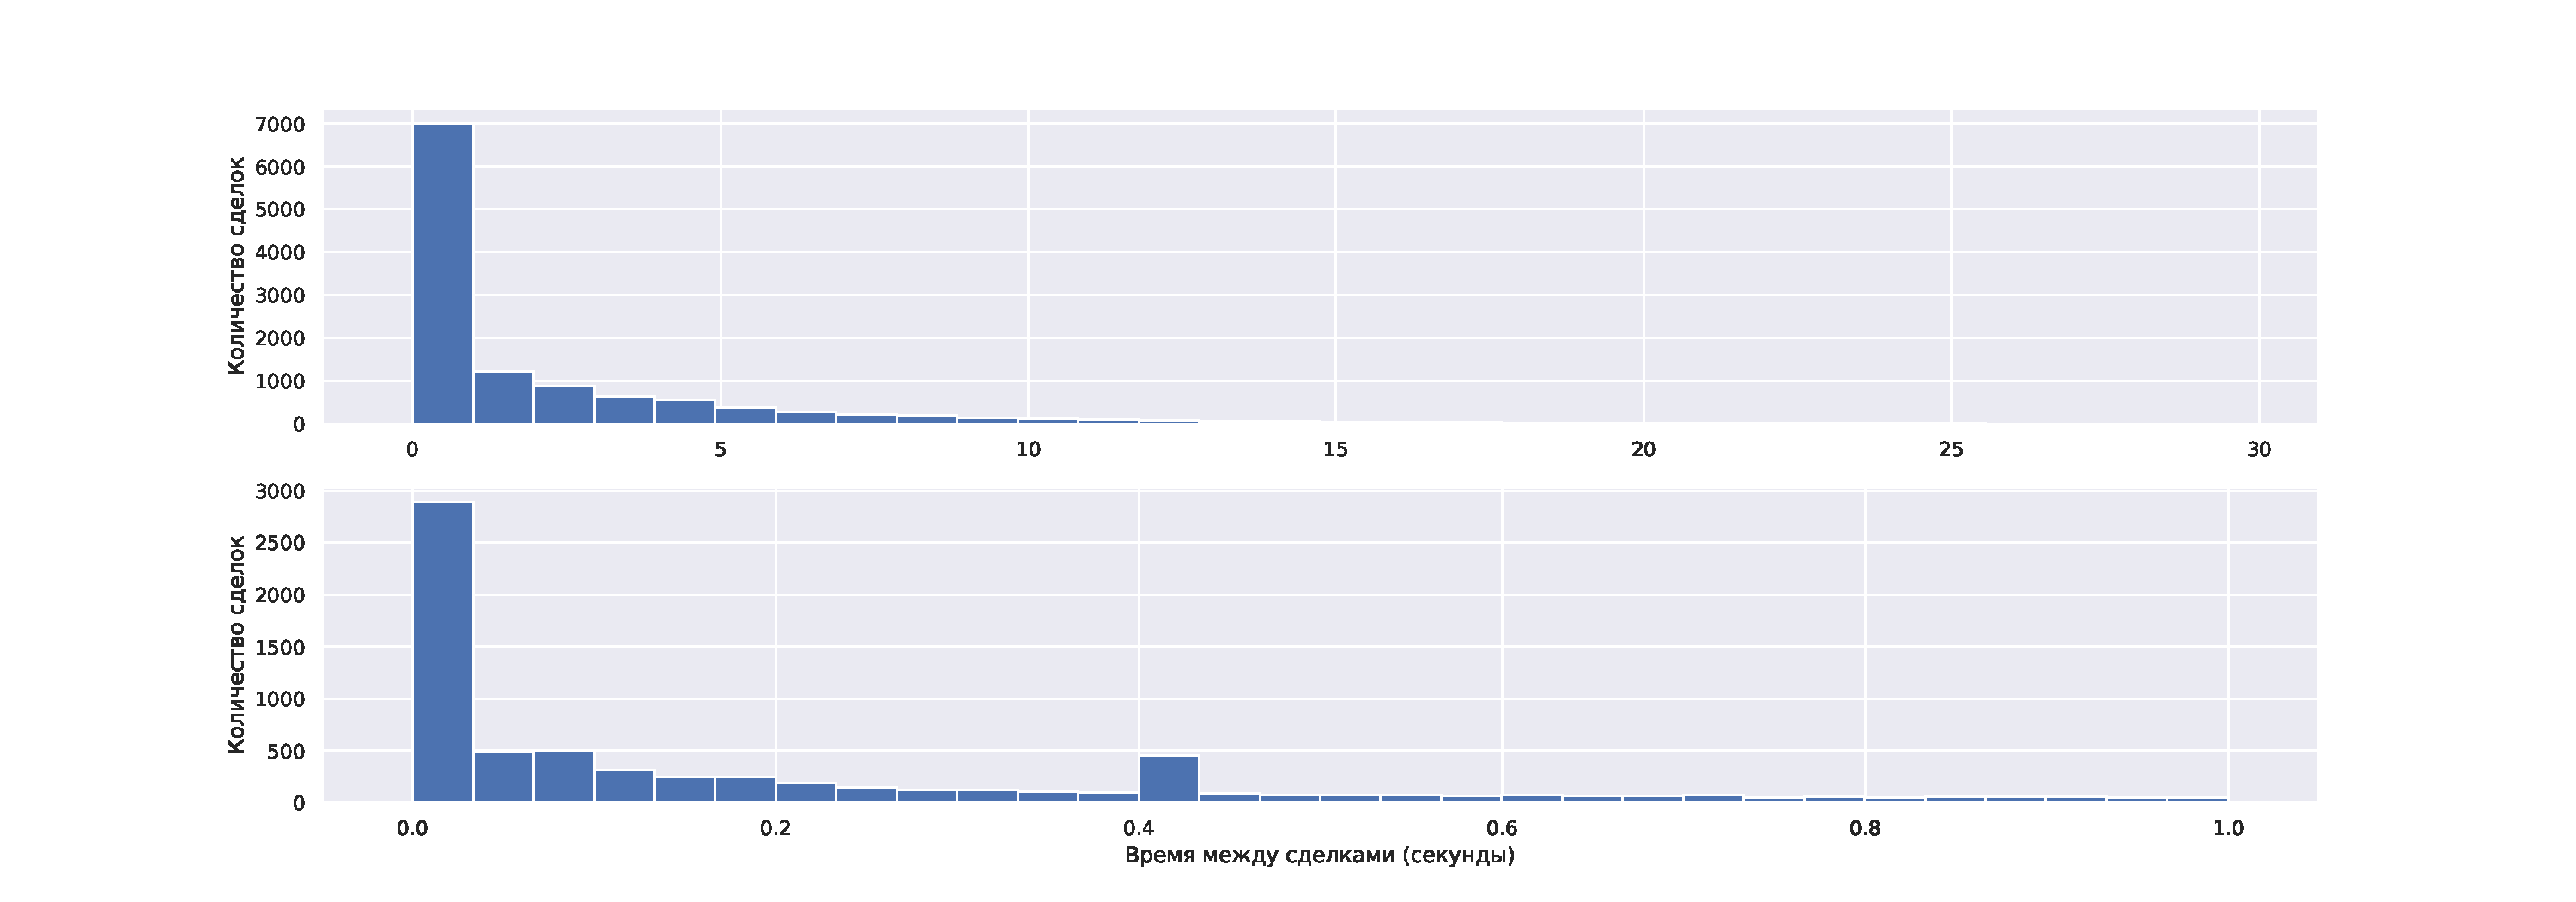
\includegraphics[scale=0.35]{fig/timedistr/SE/MGNT.pdf}
                \caption{Распределение времени между сделками для MGNT}
                \label{app}
        \end{figure}

        \begin{figure}
                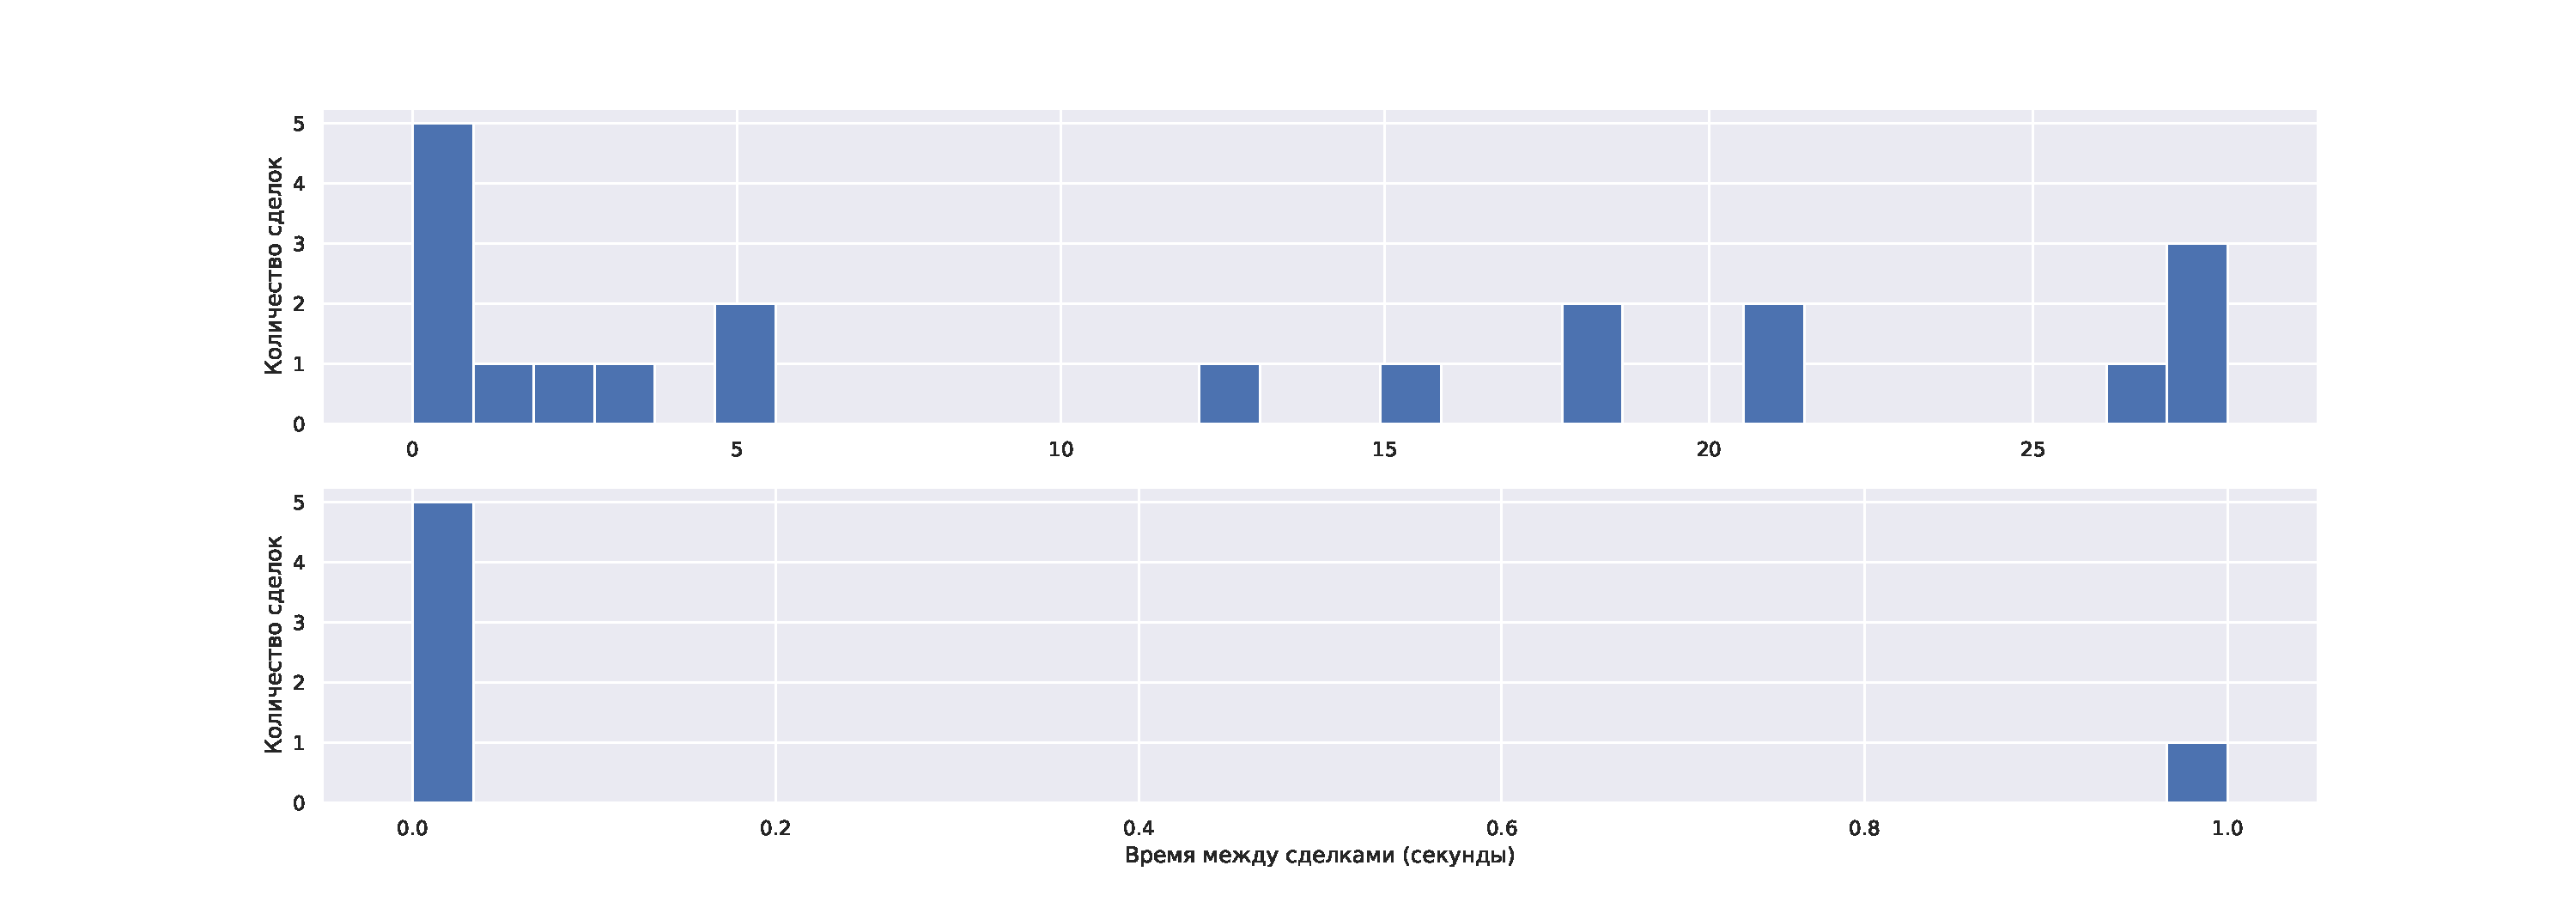
\includegraphics[scale=0.35]{fig/timedistr/CU/CNY000000TOD.pdf}
                \caption{Распределение времени между сделками для CNY000000TOD}
                \label{app}
        \end{figure}
        \begin{figure}
            \includegraphics[scale=0.35]{fig/timedistr/CU/CNYRUB\_TOM.pdf}
            \caption{Распределение времени между сделками для CNYRUB\_TOM}
            \label{app}
        \end{figure}
        \begin{figure}
                \includegraphics[scale=0.35]{fig/timedistr/CU/EUR\_RUB\_\_TOD.pdf}
                \caption{Распределение времени между сделками для EUR\_RUB\_\_TOD}
                \label{app}
        \end{figure}
        \begin{figure}
            \includegraphics[scale=0.35]{fig/timedistr/CU/EUR\_RUB\_\_TOM.pdf}
            \caption{Распределение времени между сделками для EUR\_RUB\_\_TOM}
            \label{app}
        \end{figure}
        \begin{figure}
                \includegraphics[scale=0.35]{fig/timedistr/CU/GBPRUB\_TOD.pdf}
                \caption{Распределение времени между сделками для GBPRUB\_TOD}
                \label{app}
        \end{figure}
        \begin{figure}
                \includegraphics[scale=0.35]{fig/timedistr/CU/GBPRUB\_TOM.pdf}
                \caption{Распределение времени между сделками для GBPRUB\_TOM}
                \label{app}
        \end{figure}
        \begin{figure}
                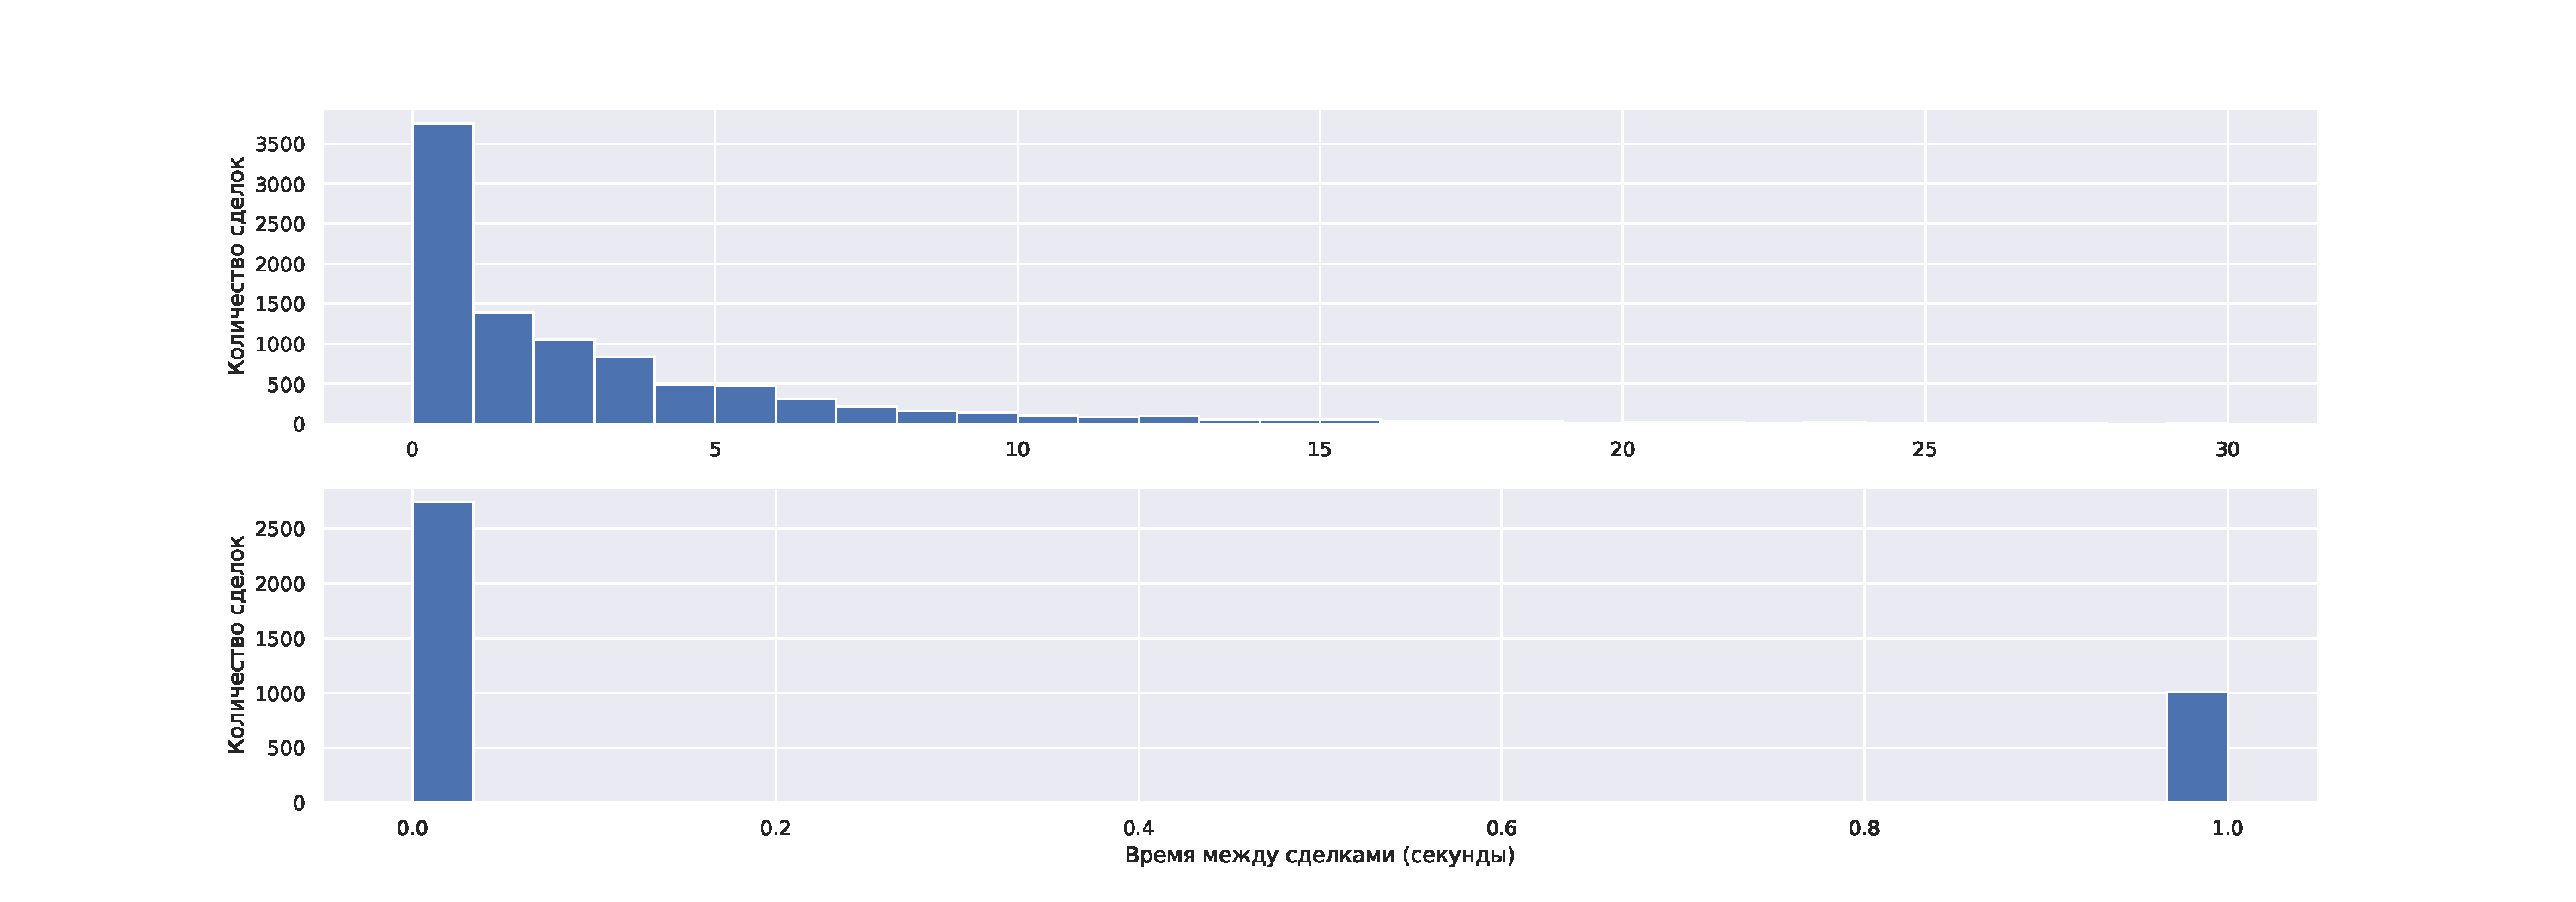
\includegraphics[scale=0.35]{fig/timedistr/CU/USD000000TOD.pdf}
                \caption{Распределение времени между сделками для USD000000TOD}
                \label{app}
        \end{figure}
        \begin{figure}
                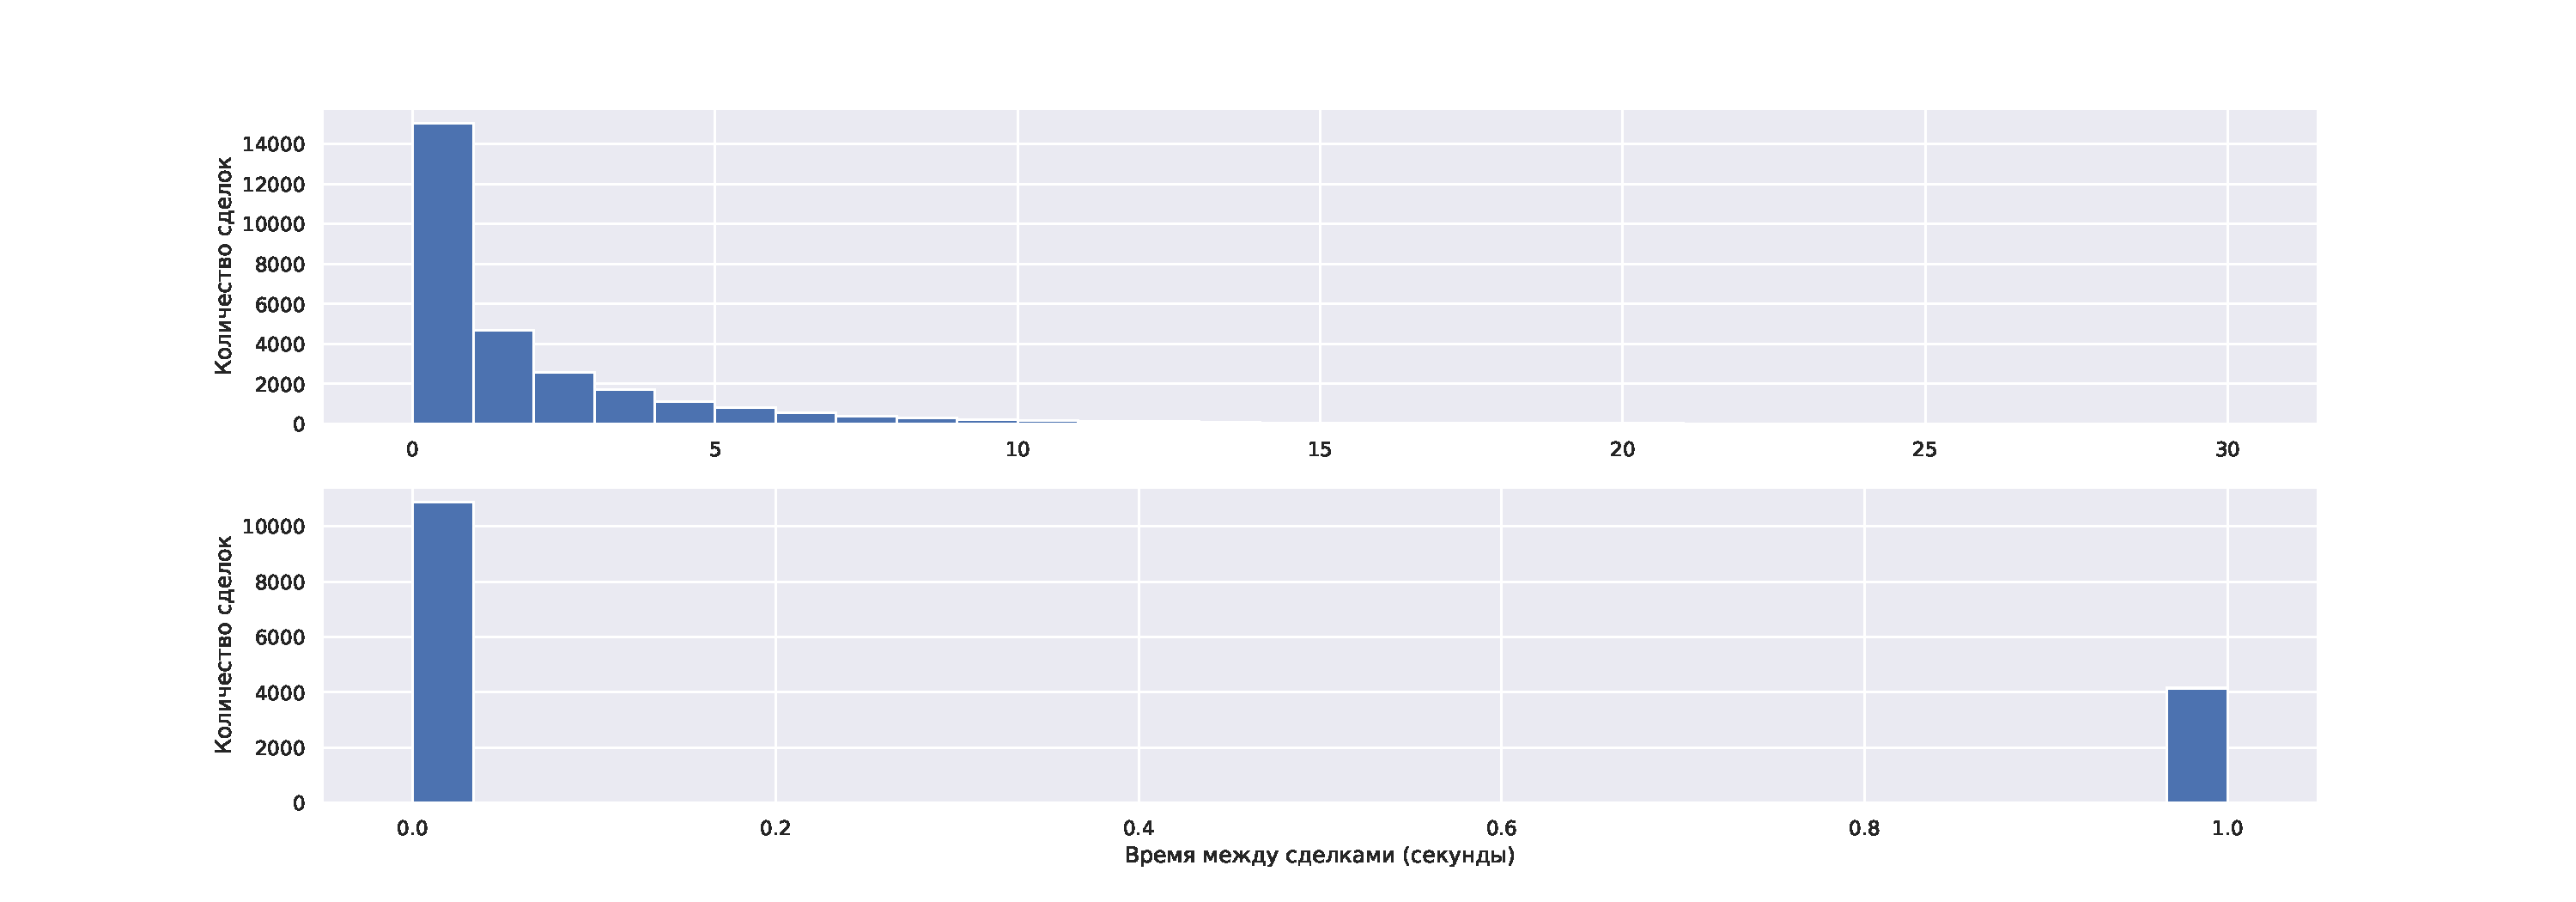
\includegraphics[scale=0.35]{fig/timedistr/CU/USD000UTSTOM.pdf}
                \caption{Распределение времени между сделками для USD000UTSTOM}
                \label{append}
        \end{figure}


        \section{Результаты регрессий на сырых данных}

        \begin{table}[h!]
                \begin{center}
                    \begin{tabular}{|c|c|c|c|c|c|}
                        \hline
                    Инструмент       & Общее число сделок & $\rho$ & $\rho ^*$ \\ \hline
                    USD000UTSTOM     & $41963$ & $63550^{***}$ & $18345^{***}$ \\ \hline
                    USD000000TOD     & $13391$ & $69906^{***}$ & $14649^{***}$ \\ \hline
                    EUR\_RUB\_\_TOM  & $13383$ & $62892^{***}$ & $2483^{***} $ \\ \hline
                    EUR\_RUB\_\_TOD  & $4134 $ & $47462^{***}$ & $1675^{**}  $ \\ \hline
                    USD000TODTOM     & $1343 $ & $19322^{***}$ & $23534^{***}$ \\ \hline
                    EURUSD000TOM     & $915  $ & $9673^{**}  $ & $4417^{*}   $ \\ \hline
                    EUR000TODTOM     & $265  $ & $6446       $ & $3750       $ \\ \hline
                    GBPRUB\_TOM      & $234  $ & $0.0053     $ & $-0.0132    $ \\ \hline
                    CNYRUB\_TOM      & $167  $ & $11214      $ & $1193       $ \\ \hline
                    \end{tabular}
                \end{center}
                \label{tableanalrdcu}
                \caption{$B$ и $B ^*$, вычисленные для разных валютных пар на сырых данных}
            \end{table} 
            
            \begin{table}[h!]
                \begin{center}
                    \begin{tabular}{|c|c|c|c|c|c|}
                        \hline
                    Инструмент        & Общее число сделок & $B$ & $B^*$ \\ \hline
                    SBER &  $41647$  & $ 43257    $ & $ 357819     $ \\ \hline
                    GAZP &  $21566$  & $ 31240^{***}    $ & $ 298196^{***}     $ \\ \hline
                %     VTBR &  $17100$  & $ 2.44e-23 $ & $ 1.49e-23 $  \\ \hline
                    YNDX &  $14110$  & $ 24715^{***}    $ & $ 65218^{***}     $ \\ \hline
                    MGNT &  $10929$  & $ 19207^{***}    $ & $ 181582^{***}    $  \\ \hline
                    LKOH &  $9759 $ &  $307474^{***}    $ & $ 151761^{***}    $  \\ \hline
                    ROSN &  $8648 $ &  $65814^{***}     $ & $ 92876^{***}     $ \\ \hline
                    PLZL &  $7121 $ &  $11072^{***}     $ & $ 267550^{***}    $  \\ \hline
                    SNGSP & $ 6032$  & $ 8652^{***}     $ & $ 137911^{***}    $  \\ \hline
                    MTLR &  $5985 $ &  $5031^{***}      $ & $ 59414^{***}     $ \\ \hline
                    \end{tabular}
                \end{center}
                \label{tableanalrdse}
                \caption{$B$ и $B ^*$, вычисленные для разных акций на сырых данных}
            \end{table} 
            В данном случае нет формальных оснований полагать, что полученные числа 
            (см. таблицы \ref{tableanalrdcu} и \ref{tableanalrdse}) имеют какое бы то ни было отношение к модели 
            Обижаевой--Ванга. Однако, прослеживается некоторая связь между ликвидностью актива и величиной $\rho$, так что есть 
            вероятность того, что они всё же являются осмысленной мерой ликвидности, связанной с моделью. 
            Возможно, развитие идей, высказанных в разделе \ref{AppendixBigRho}, помогло бы установить связь между вычисленными в регрессии
            коэффициентами $B$ и $\rho$. 
\end{appendices}   % Do not change this line